\section{Implementation of systematic uncertainties}
\subsection{Variation of Detector Properties}
\label{sec:detector-unc}
Systematic uncertainties on the detector properties that need to be taken into account are the overall optical efficiency of the DOMs as well as the properties of the surrounding ice.
The parametrization and priors of each of these properties are informed by IceCube calibration studies.
\begin{itemize}
    \item DOM efficiency: A factor that scales the probability that a photon hitting the PMT of a DOM will produce a photo-electron that is measured by the electronics.
Nominal value is 1, prior standard deviation is 10\%.
    \item Hole ice: Two parameters describe the effect of the optical properties of the column of re-frozen ice within the bore holes in which the strings have been deployed.
The details of this parametrization is described below.
    \item Bulk ice: The over-all absorption and scattering coefficients of all ice layers are multiplied by a scaling factor.
The nominal value for ice absorption is 1.0 with a prior standard deviation of 5\%.
The nominal value for ice scattering is 1.05 with a prior standard deviation of 10\%.
\end{itemize}

In total, the uncertainties on the detector properties are modeled by five  parameters, one for the DOM efficiency, two for the hole ice model and two for the bulk ice uncertainty.
To model the effect of these parameters on the analysis histogram, several MC sets at different variations of DOM efficiency, hole ice, and bulk ice parameters are produced.
These MC sets are used to find a parametrization that will model how the distribution of events in energy, zenith and PID will change as a function of these parameters.

\subsubsection{DOM efficiency calibration}
\label{sec:domeff-calibration}
As described in \refsec{dom-daq}, the DOMs contain LEDs that are used to calibrate the detector \emph{in-situ}. However, these LEDs are not calibrated with respect to their absolute brightness and therefore are not suited for the calibration of the optical efficiency of the DOMs. Instead, minimally ionizing muons that are produced in air showers are used as a light source with a known brightness. The calibration is performed using a sample of events that pass the \emph{Minimum Bias Trigger}\cite{icecube_detector_17} and in which the reconstructed muon track stops within the instrumented volume of IceCube. The DOM efficiency is estimated by comparing the observed charges in the DOMs and the light expectation from the reconstructed muons. Multiple such calibration studies have been run \sidecite{domeff_nick}\sidecite{domeff_jake} and found variations in the optical efficiency of approximately 10\%, which is used as a prior for the measurements presented in this work.

\subsubsection{Hole Ice Parametrization}
\label{sec:hole-ice-parametrization}

The bore holes in which IceCube's strings have been deployed were drilled using hot water to melt a column of ice into which the strings with their attached optical sensors could be lowered.
This water column re-froze after deployment to form what is referred to as \emph{hole ice}\sidecite{Fiedlschuster:2019unl}.
Camera observations of this re-freezing process suggest that the hole ice is transparent near the edges of be hole and contains a bubble column in its center\sidecite{rongen2016measuring}.
The bubble column has a much shorter scattering length than the surrounding bulk ice and therefore decreases the probability of a photon entering a DOM directly from below.
The effect of the re-frozen ice column surrounding the strings can be modeled as a modification to the optical efficiency of the DOMs as a function of the incident angle of incoming photons.
In the past, many different angular acceptance curves have been produced from \emph{in-situ} calibration measurements\cite{flasher_calibration}, the best fit results of previous DeepCore oscillation analyses, in addition to the laboratory measurements that have been made in water tanks before the deployment of IceCube.
For the analysis presented in this work, a two-dimensional parametrization was developed that can approximate any of these hole ice models such that it can be used as a \emph{unified} hole ice model.
To do this, all previous angular acceptance curves are evaluated as a function of the cosine of the photon incidence angle, $\cos(\eta)$, at 100 points over the entire valid domain between -1 and 1, where 1 represents a photon entering a DOM directly from below.
The curves are furthermore normalized to an area of 1 to avoid affecting the total observed charge.
Using Principal Component Analysis\sidecite{pca}, the variations between the different models are decomposed into a mean and the most important components that explain the variance between models.
It was found that the two most important components, $p_0$ and $p_1$, describe all known hole ice models adequately.
Their effect is shown in \reffig{hole-ice-parametrization} as variations with the acceptance curve that is used as the baseline in this analysis.
The right panel of \reffig{hole-ice-parametrization} also shows where the older hole ice models are located in the space spanned by $p_0$ and $p_1$.
The laboratory measurement, which did not include any hole ice effects, notably lies far outside of the region of all other hole ice models that are all produced \emph{in-situ}.

\begin{figure*}
    \centering
    \tikzsetnextfilename{hole_ice_p0_p1}%
\begin{tikzpicture}

\pgfplotstableread{figures/measurement/systematics/detector/hole_ice/angsens_example_fluct.csv}\table
\pgfplotstableread{figures/measurement/systematics/detector/hole_ice/all_acceptance_curves.csv}\acceptancecurves

\begin{axis}[
        width=0.45\linewidth, height=0.4\linewidth,
		xmajorgrids, ymajorgrids,
		xlabel=$\cos(\eta)$, ylabel=relative optical efficiency,
		legend style={at={(0.02,0.95)}, anchor=north west},
        ytick distance=0.2,
	]
    \addplot[black, thick] table [x=cos_theta, y=baseline] \acceptancecurves;
    \addlegendentry{baseline}
    
    \addplot[vermilion, thick] table [x=cos_theta, y=nominal] \acceptancecurves;
    \addlegendentry{laboratory}
    
    % \addplot[bluishgreen, thick] table [x=cos_theta, y=bfp_three_flav] \acceptancecurves;
    % \addlegendentry{best fit}
    
    \addplot[blue, thin, name path=fluct_p0_dn, forget plot] table [x=cos_theta, y=fluct_p0_dn] \table;
    \addplot[blue, thin, name path=fluct_p0_up, forget plot] table [x=cos_theta, y=fluct_p0_up] \table;
    \addplot[blue, opacity=0.5] fill between[of = fluct_p0_dn and fluct_p0_up];
    \addlegendentry{example variation in $p_0$}
    
    \addplot[orange, thin, name path=fluct_p1_dn, forget plot] table [x=cos_theta, y=fluct_p1_dn] \table;
    \addplot[orange, thin, name path=fluct_p1_up, forget plot] table [x=cos_theta, y=fluct_p1_up] \table;
    \addplot[orange, opacity=0.5] fill between[of = fluct_p1_dn and fluct_p1_up];
    \addlegendentry{example variation in $p_1$}
	
\end{axis}
\end{tikzpicture}
    \tikzsetnextfilename{hole_ice_models_scatter}%
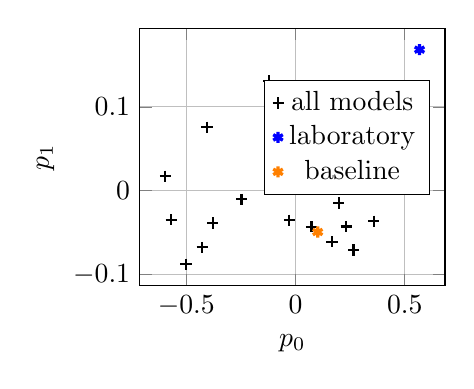
\begin{tikzpicture}
\begin{axis}[
        width=0.45\linewidth, height=0.4\linewidth,
		xmajorgrids, ymajorgrids,
		xlabel=$p_0$,
		ylabel=$p_1$,
		legend columns=1,
		legend style={
			/tikz/every even column/.append style={column sep=0.2cm},
			at={(0.95, 0.8)},
			anchor=north east
		}
        % ytick={-0.1, -0.05, 0, 0.05, 0.1},
        % yticklabels={-0.1, -0.05, 0, 0.05, 0.1}
	]
    \addplot[black, only marks, mark=+, thick] table [x=p0, y=p1] {
       	name	p0	p1
        %nominal	0.567771	0.168269
        h1-100cm	-0.123027	0.131104
        h2-50cm	-0.405128	0.075841
        h3-30cm	-0.595997	0.017468
        dima	0.232258	-0.042754
        dima+	0.265798	-0.070837
        dima-	0.198792	-0.014733
        dragon	0.072961	-0.043175
        greco	0.167150	-0.060809
        %baseline	0.101569	-0.049344
        msu2	0.357705	-0.036428
        martin-0.6-14	-0.028113	-0.035254
        martin-0.8-40	-0.246929	-0.010401
        martin-1.8-125	-0.569511	-0.034839
        all	-0.427318	-0.067581
        tilted	-0.501349	-0.087664
        horizontal	-0.378935	-0.038564
    };
    \addlegendentry{all models}
    \addplot[blue, only marks, mark=asterisk, very thick] coordinates {
        (0.567771,	0.168269)
    };
    \addlegendentry{laboratory}
    \addplot[orange, only marks, mark=asterisk, very thick] coordinates {
        (0.101569,	-0.049344)
    };
    \addlegendentry{baseline}
    

	
\end{axis}
\end{tikzpicture}
    \caption{Two parameter model used to parametrize the optical efficiency in this analysis (left) and the positions in this two-dimensional space where older hole ice models are located (right). The relative optical efficiency curves are normalized to have the same area, which can lead to acceptance values greater than 1.}
    \label{fig:hole-ice-parametrization}
\end{figure*}

\subsubsection{Depth-dependent ice properties}
\label{sec:depth-dependent-ice-properties}

In the parametrization of the uncertainties of the detector properties described in \refsec{detector-unc}, variations of the scattering and absorption coefficients are only described by global, depth-independent scaling factors.
In principle, the error on the properties of the ice can also change as a function of depth.
Such variations are expected because regions of higher absorption and scattering coefficients will also absorb and scatter the light from the LED flashers that is used to do the calibration.
Higher uncertainties are also expected near the edges of the detector since there are no more calibration light sources outside of the instrumented volume.
Of particular interest for the analysis presented in this work are variations of the ice properties at length scales of the DeepCore fiducial volume located within DeepCore.
Variations at much longer scales would be indistinguishable from uniform variations given the size of the event signatures observed below 100~GeV, while variations at much shorter scales are expected to average out.
To test how significantly such a variation would impact the final level histograms, two MC sets are produced in which the scattering and absorption coefficients vary following a sigmoid function centered in DeepCore with an amplitude of $\pm 2\%$ in opposing directions as shown in \reffig{step-function-ice-model}.
\begin{figure}
    \centering
    \tikzsetnextfilename{ice_step_func_perturbations}%
\begin{tikzpicture}
\begin{axis}[
    height=0.5\linewidth,
    width=0.8\linewidth,
    xmin=1100,xmax=2900,
    xticklabel style={/pgf/number format/.cd,1000 sep={}},
    ymin=0.97, ymax=1.03,
    enlarge y limits=true,
    xlabel=depth (m),
    legend columns=2,
    ylabel=perturbation factor,
    xmajorgrids, ymajorgrids
]
    \addplot[black, thick] table [x=depth, y=perturbation1, col sep=comma] {figures/measurement/systematics/detector/ice_perturbation/ice_perturbations.csv};
    \addlegendentry{perturbation +2\%}
    
    \addplot[orange, thick] table [x=depth, y=perturbation2, col sep=comma] {figures/measurement/systematics/detector/ice_perturbation/ice_perturbations.csv};
    \addlegendentry{perturbation -2\%}
    % dust layer
    \draw [name path=dust layer top, gray, thin] (2000, \pgfkeysvalueof{/pgfplots/ymin}) -- (2000, \pgfkeysvalueof{/pgfplots/ymax}); 
    \draw [name path=dust layer bottom, gray, thin] (2100, \pgfkeysvalueof{/pgfplots/ymin}) -- node[sloped, above, black, font=\footnotesize\sffamily] {dust layer} (2100, \pgfkeysvalueof{/pgfplots/ymax});
    \addplot [gray, opacity=0.4] fill between [of=dust layer top and dust layer bottom];
    
    % IceCube
    \draw [name path=icecube top, gray, thin] (1450, \pgfkeysvalueof{/pgfplots/ymin}) -- (1450, \pgfkeysvalueof{/pgfplots/ymax}); 
    \draw [name path=icecube bottom, gray, thin] (2000, \pgfkeysvalueof{/pgfplots/ymin}) -- (2000, \pgfkeysvalueof{/pgfplots/ymax});
    \node[anchor=south, black, font=\footnotesize\sffamily] at (1750, 0.97) {IceCube\strut};
    \addplot [gray, opacity=0.2] fill between [of=icecube top and icecube bottom];
    
    % DeepCore
    \draw [name path=deepcore top, gray, thin] (2100, \pgfkeysvalueof{/pgfplots/ymin}) -- (2100, \pgfkeysvalueof{/pgfplots/ymax}); 
    \draw [name path=deepcore bottom, gray, thin] (2450, \pgfkeysvalueof{/pgfplots/ymin}) -- (2450, \pgfkeysvalueof{/pgfplots/ymax});
    \node[anchor=south, black, font=\footnotesize\sffamily] at (2270, 0.97) {DeepCore\strut};
    \addplot [gray, opacity=0.1] fill between [of=deepcore top and deepcore bottom];
    
\end{axis}

\end{tikzpicture}

    \caption{Perturbation of the scattering and absorption coefficients with respect to the nominal ice model applied in additional MC sets.}
    \label{fig:step-function-ice-model}
\end{figure}
The size of this variation corresponds approximately a $1\sigma$-allowed variation according to flasher calibration data.
For every bin in the final analysis histogram, a linear regression is fit to the bin counts of the nominal MC set and the two variations.
By comparing the $\chi^2$ test statistic resulting from the regression with the free fit and a regression where the slope is fixed to zero, a p-value can be calculated for every bin, where the null hypothesis is that the step-function variation has no effect.
The p-values for all analysis bins are shown in \reffig{steppiness-pvals} and are consistent with random fluctuations.
Therefore, it was concluded that the effect of a depth-dependent ice model variation is well within the statistical uncertainty of the simulation and need not be included in the measurement.
\begin{figure}
    \centering
    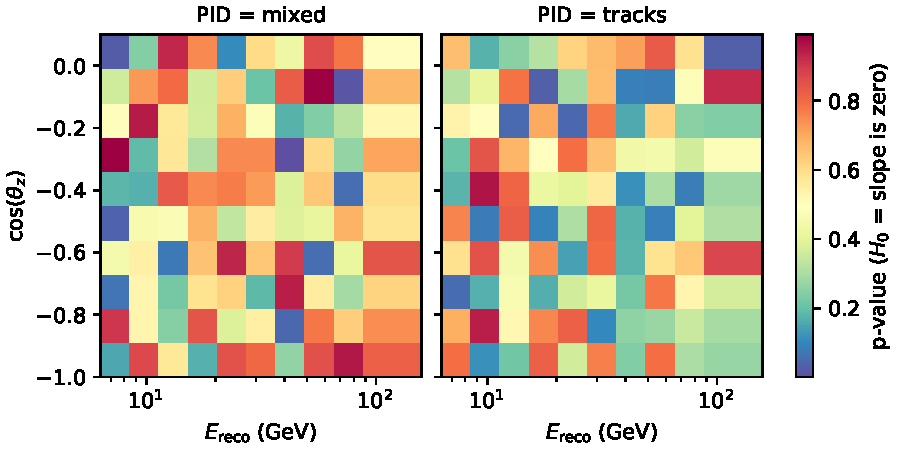
\includegraphics[width=0.9\linewidth]{figures/measurement/systematics/detector/ice_perturbation/steppiness_slope_pvals_verification_sample.pdf}
    \caption{Bin-wise p-value of the fitted slopes as a function of the step-function ice model variation.}
    \label{fig:steppiness-pvals}
\end{figure}

\subsection{Variation of the Atmospheric Neutrino Flux}
\label{sec:flux_systs}

The atmospheric neutrino flux can vary depending on the choice of primary cosmic ray (CR) model, assumed meson yield, hadronic interaction (HI) model and atmospheric density model that are used in the calculation.
The nominal flux, $\Phi_\mathrm{nom}$, is modified to a systematic flux, $\Phi_\mathrm{sys}$, so that

\begin{equation}
    \Phi_{\mathrm{sys}}(E) = \Phi_{\mathrm{nom}} \cdot \left( \frac{E}{E_\mathrm{pivot}}\right)^{\Delta \gamma}
    +
    \sum_{i=1}^{N_\mathrm{Barr}} B_i \cdot \frac{\mathrm{d} \Phi_{\mathrm{nom}}}{\mathrm{d}B_i}\label{eq:flux-variation}
\end{equation}

The $\Delta \gamma$ in \refeq{flux-variation} is due to the CR flux uncertainty and corresponds to shifting the spectral index of the neutrino flux, with a pivot point at $E_\mathrm{pivot}=24\;\mathrm{GeV}$. The second term describes the uncertainty of the Pion and Kaon production yield, where each $B_i$ corresponds to the variation in one \emph{Barr block} (further described below). The gradients with respect to these variations, $\frac{\mathrm{d} \Phi_{\mathrm{nom}}}{\mathrm{d}B_i}$, are calculated using the \textsc{MCEq}\cite{mceq, fedynitch2012influence,fedynitch2015calculation} flux calculator.

\subsubsection{Uncertainty on Meson Production}
\labsec{barr-scheme}
The Barr scheme\sidecite{Barr2006} entails dividing the phase space of incident parent particle $E_\mathrm{i}$ and the outgoing secondary particle $E_\mathrm{s}$ (or, equivalently, $x_{\mathrm{LAB}}=E_\mathrm{s}/E_\mathrm{i}$) into regions that are each denoted by a Barr variable.
There are eight regions/variables that define the uncertainty on $ \pi^+ $ production, and four regions that define the $K^+$ production, as shown in \reffig{barr-blocks}.
For every region, a different relative uncertainty is assigned based on the experimental constraints in that region, as shown in \reffig{barr-blocks-uncertainty}.
For primary particle energies $>500\;\mathrm{GeV}$, an additional energy-dependent term is added to the uncertainty to account for the fact that no accelerator measurements are available at these energies to constrain the meson yield.
As the pion ratio is well-measured, the uncertainty on $ \pi^- $ is defined by the uncertainty on $ \pi^+ $ combined with the uncertainty on the pion ratio.
The uncertainty on $ K^- $ production is parametrized separately from the $K^+$ production.
The only modification to the original Barr scheme used in this analysis is that the low-energy $ \pi^+ $ Barr variables A-F are summarized to a single variable with a relative uncertainty of 63\%, because their impact was found to be highly correlated.
Thus the uncertainty from meson production is described by $N_\mathrm{Barr}=17$ Barr variables that enter \refeq{flux-variation}.

\begin{figure}
    \centering
    \tikzsetnextfilename{barr_blocks_annotated}%
\begin{tikzpicture}
    \node[above right, inner sep=0] (image) at (0,0) {
        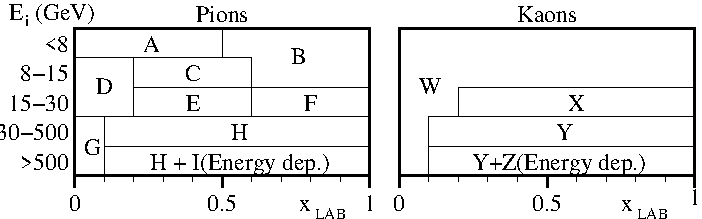
\includegraphics[width=0.8\linewidth]{figures/measurement/systematics/flux/barr_blocks.pdf}
    };
    % Create scope where axes are matching the Pion grid
    \begin{scope}[
        x={($0.42*(image.south east)$)},
        y={($0.67*(image.north west)$)},
        shift={($0.107*(image.south east) + 0.2*(image.north west)$)}
    ]
        % Grid
        %\draw[darkgray,step=0.2] (0,0) grid (1,1);
        \draw[thick, orange, fill=orange, fill opacity=0.8] (0, 0.4) rectangle (1, 1);
        \node[anchor=south, fill=white, draw=black] at (0.5, 0.55) {merged A-F};
    \end{scope}
\end{tikzpicture}
    %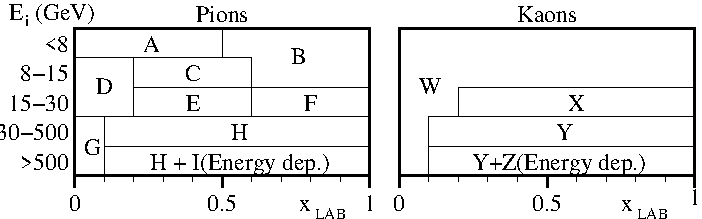
\includegraphics[width=0.8\linewidth]{figures/measurement/systematics/flux/barr_blocks.pdf}
    \caption{Fully correlated regions of uncertainties in the hadronic interaction model. Figure taken from \cite{Barr2006}.}
    \labfig{barr-blocks}
\end{figure}
\begin{figure}
    \centering
    \tikzsetnextfilename{barr_blocks_uncertainty_annotated}%
\begin{tikzpicture}
    \node[above right, inner sep=0] (image) at (0,0) {
        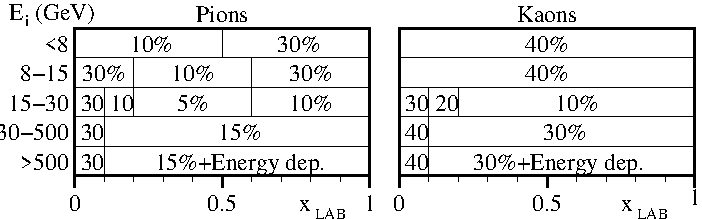
\includegraphics[width=0.8\linewidth]{figures/measurement/systematics/flux/barr_blocks_uncertainty.pdf}
    };
    % Create scope where axes are matching the Pion grid
    \begin{scope}[
        x={($0.42*(image.south east)$)},
        y={($0.67*(image.north west)$)},
        shift={($0.107*(image.south east) + 0.2*(image.north west)$)}
    ]
        % Grid
        %\draw[darkgray,step=0.2] (0,0) grid (1,1);
        \draw[thick, orange, fill=orange, fill opacity=0.8] (0, 0.4) rectangle (1, 1);
        \node[anchor=south, fill=white, draw=black] at (0.5, 0.55) {63\%};
    \end{scope}
\end{tikzpicture}
    %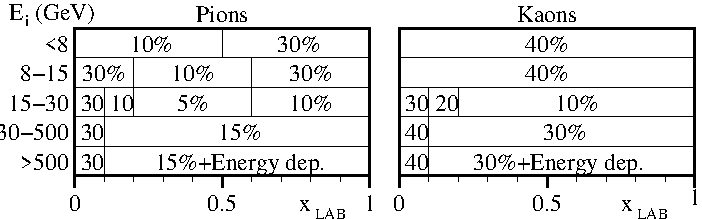
\includegraphics[width=0.8\linewidth]{figures/measurement/systematics/flux/barr_blocks_uncertainty.pdf}
    \caption{Relative uncertainty assigned to each region of hadron phase space in percent. Figure taken from \cite{Barr2006}.}
    \labfig{barr-blocks-uncertainty}
\end{figure}

%Only in the sterile analysis, the prior on the variables with an energy-dependent uncertainty, \texttt{barr\_i\_Pi}, \texttt{barr\_z\_K}, and \texttt{barr\_z\_antiK} by a factor of 5 to 0.61, because it was found that the original priors used in the standard three-flavor analysis greatly under-estimated the impact of these parameters compared to the original Barr 2006 paper.

\subsubsection{Atmospheric density}

The development of particle showers in the atmosphere is governed by competing processes of decay and interactions with the surrounding air.
The density of the atmosphere can therefore influence the rate of neutrino production and could potentially contribute a systematic uncertainty to oscillation measurements.
The size of the effect of atmospheric density uncertainty on the analysis presented in this work is estimated using the same procedure as described in \cite{MEOWS}.
This is done by obtaining a variation of atmospheric density profile by perturbing the Earth’s atmospheric temperature within a prior range given by the NASA Atmospheric InfraRed Sounder (AIRS) satellite~\cite{AIRS} temperature data.
The resulting atmospheric density profile are injected into \textsc{MCEq} to calculate new fluxes.
This is performed for a variety of CR models and hadronic interaction models available in \textsc{MCEq}.
The resulting fluctuations of the neutrino flux observed at the detector were found to be consistently below 1\% for the energy ranges most relevant to DeepCore measurements and is therefore not included as a systematic uncertainty in this work.

